\ifx\wholebook\relax \else

\documentclass[b5paper]{ctexart}
\usepackage[nomarginpar
  %, margin=.5in
]{geometry}

\addtolength{\oddsidemargin}{-0.05in}
\addtolength{\evensidemargin}{-0.05in}
\addtolength{\textwidth}{0.1in}

\usepackage[cn]{../../../prelude}

\setcounter{page}{1}

\begin{document}

\title{列表}

\author{刘新宇
\thanks{{\bfseries 刘新宇} \newline
  Email: liuxinyu95@gmail.com \newline}
  }

\maketitle
\fi

\markboth{列表}{基本算法}

\ifx\wholebook\relax
\chapter{列表}
\numberwithin{Exercise}{chapter}
\fi

\section{简介}
\label{introduction}

列表和数组是构建其它复杂数据结构的基石。它们都可以看作是容纳若干元素的容器。数组通常是一组连续的存储区域,每个存储单元由一个数字索引。这个数字叫作地址或者位置。数组的大小是有限的,通常需要在使用前确定。与数组不同,列表的大小无需预先确定,可以随时加入新元素。我们可以从头到尾依次遍历列表中的元素。特别是在函数式环境中,列表相关算法对于计算和逻辑的控制起着关键作用\footnote{在更底层,lambda演算作为和图灵机等价的计算模型更为基础\cite{mittype}, \cite{unplugged}。}。对于已经熟悉映射(map),过滤(filter),叠加(fold)等算法的读者,可以跳过这一章,直接从第二章开始阅读。

\section{定义}
\index{列表!定义}

列表又称单向链表,是一种递归的数据结构。其定义如下:

\begin{itemize}
\item 一个\textbf{列表}或者为空,记为 $\nil$或NIL;
\item 或者包含一个元素和一个\textbf{列表}。
\end{itemize}

图\ref{fig:list-example}描述了一个由若干节点组成的列表。每个节点包含两部分,一个元素(也称作key)和一个子列表。指向子列表的引用通常叫作next。最后一个节点中的子列表为空,记为‘NIL’。

\begin{figure}[htbp]
  \centering
    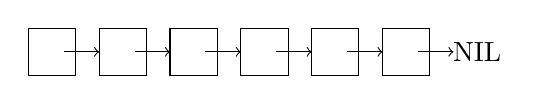
\begin{tikzpicture}[scale=3]
    \foreach \x in {-2, -1.7, ..., -0.4} {
      \draw (\x cm, 1cm) +(-0.1, -0.1) rectangle ++(0.1, 0.1);
      \draw[->] (\x cm, 1cm) +(0.05, 0) -- +(0.2, 0);
    }
    \draw (-0.2cm, 1cm) node {NIL};
    \end{tikzpicture}
  \caption{由节点组成的列表}
  \label{fig:list-example}
\end{figure}

每个节点要么链接到下一个节点上,要么指向NIL。通常使用复合数据结构\footnote{多数情况下,列表中元素有着共同的类型。有些环境(如Lisp)支持包含不同数据类型的列表。}定义列表,例如:

\lstset{frame=single}
\begin{lstlisting}[language=Bourbaki]
struct List<A> {
    A key
    List<A> next
}
\end{lstlisting}

\index{列表!空} \index{列表!判空}

这里需要对“空”列表的概念加以说明。很多传统的编程环境支持空引用null概念,因此存在两种不同的方法表示空列表。一种直接使用空引用null(或NIL);另一种创建一个列表,但不填入任何元素,通常表示为\texttt{[]}。在实现上,空引用无需占用内存,但\texttt{[]}则需要分配内存。本书使用符号$\varnothing$表示抽象的空列表、空集、空容器。

\subsection{分解}
\index{列表!头} \index{列表!尾} \index{列表!构造} \index{列表!cons}

给定一个非空列表$L$,我们定义两个函数来分别获取头部元素和子列表。它们通常被命名为$first(L)$和$rest(L)$,或者$head(L)$和$tail(L)$\footnote{在Lisp中,由于历史原因,它们被命名为\texttt{car}和\texttt{cdr}用以代表当时机器中的寄存器\cite{SICP}}。反之,我们可以从一个元素$x$和列表$xs$(可为空)构造出另一个列表,记为$x : xs$。这一构造过程也叫作\texttt{cons}。我们有如下关系:

\be
\begin{cases}
head(x:xs) & = x \\
tail(x:xs) & = xs
\end{cases}
\label{eq:list-head-tail}
\ee

对于非空列表$X$,我们也用$x_1$表示第一个元素,用$X'$表示剩余列表,例如$X = [x_1, x_2, x_3, ...]$,$X' = [x_2, x_3, ...]$。

\begin{Exercise}
\Question{对于元素类型为$A$的列表,如果能够判断任何两个元素$x, y \in A$是否相等,定义一个算法来判断两个列表是否相等。}
\end{Exercise}

\subsection{列表的基本操作}
\index{列表!长度}
根据定义,我们可以递归地计算列表的长度:空列表的长度为0,而非空列表的长度是除去第一个元素的子列表长度加一。

\be
\begin{array}{rcl}
length(\nil) & = & 0 \\
length(L) & = & 1 + length(L')
\end{array}
\ee

为了计算长度,我们从头到尾遍历列表。其时间复杂度是$O(n)$,其中$n$是元素个数。为了避免反复计数,我们可以将长度存储在一个变量中,并在增加或删除元素时更新这一变量。下面是计算长度的迭代实现:

\begin{algorithmic}[1]
\Function{Length}{L}
  \State $n \gets 0$
  \While{$L \neq $ NIL}
    \State $n \gets n + 1$
    \State $L \gets $ \Call{Next}{$L$}
  \EndWhile
  \State \Return $n$
\EndFunction
\end{algorithmic}

在不和绝对值混淆的情况下,我们也使用$|L|$来表示列表$L$的长度。

\subsection{索引}
\index{列表!索引(get at)}

数组支持以常数时间随机访问任意位置$i$的元素。但列表需要前进$i$步才能到达元素所在位置。

\be
getAt(i,\ x:xs) = \begin{cases}
  i = 0: & x \\
  i \neq 0: & getAt(i - 1, xs) \\
\end{cases}
\ee

为了从一个非空列表中获取第$i$个元素:
\begin{itemize}
\item 若$i$为0,结果为列表中的头部元素;
\item 否则,结果为子列表中的第$i-1$个元素。
\end{itemize}

我们故意没有处理空列表的情况。如果传入$\nil$,此时的行为是未定义的。$i$越界时的行为也是未定义的。若$i > |L|$,通过递归,最终转化为访问空列表的第$i - |L|$个位置的情况。另一方面,若$i < 0$,继续减一将使得它更偏离0,最终转化为访问空列表的某个负索引位置的情况。

由于需要前进$i$步,索引算法的时间复杂度为$O(i)$。下面是对应的迭代实现:

\begin{algorithmic}[1]
\Function{Get-At}{$i, L$}
  \While{$i \neq 0$}
    \State $L \gets $ \Call{Next}{$L$}  \Comment{$L$ = NIL时出错}
    \State $i \gets i - 1$
  \EndWhile
  \State \Return \Call{First}{$L$}
\EndFunction
\end{algorithmic}

\begin{Exercise}
\Question{在\textproc{Get-At}($i, L$)的迭代实现中,$L$为空会怎样?$i$越界时会怎样?}
\end{Exercise}

\subsection{末尾元素}
\index{列表!末尾元素} \index{列表!init}

存在一对和first/rest对称的操作,称为last/init。对于非空列表$X = [x_1, x_2, ..., x_n]$,函数$last$返回末尾元素$x_n$,而$init$返回子列表$[x_1, x_2, ..., x_{n-1}]$。虽然这两对操作左右对称,但last/init需要遍历列表,因而是线性时间的。

当获取列表$X$的末尾元素时:

\begin{itemize}
\item 如果列表只含有一个元素$[x_1]$,则$x_1$就是末尾元素;
\item 否则,结果为子列表$X'$的末尾元素。
\end{itemize}

\be
\begin{array}{rcl}
last([x]) & = & x \\
last(x:xs) & = & last(xs) \\
\end{array}
\label{eq:list-last}
\ee

类似地,当获取除去末尾元素的子列表时:

\begin{itemize}
\item 如果列表只含有一个元素$[x_1]$,结果为空$[\ ]$;
\item 否则,我们递归地从子列表$X'$中获取除去末尾元素的剩余部分,然后将$x_1$附加在前面。
\end{itemize}

\be
\begin{array}{rcl}
init([x]) & = & [\ ] \\
init(x:xs) & = & x : init(xs) \\
\end{array}
\ee

这两个算法中都没有处理空列表的情况,当传入$\nil$时,其行为是未定义的。下面是相应的迭代实现。

\begin{algorithmic}[1]
\Function{Last}{$L$}
  \State $x \gets $ NIL
  \While{$L \neq$ NIL}
    \State $x \gets $ \Call{First}{$L$}
    \State $L \gets $ \Call{Rest}{$L$}
  \EndWhile
  \State \Return $x$
\EndFunction
\Statex
\Function{Init}{$L$}
  \State $L' \gets $ NIL
  \While{\Call{Rest}{$L$} $\neq$ NIL} \Comment{$L$为NIL时出错}
    \State $L' \gets$ \textproc{Cons}(\Call{First}{$L$}, $L'$)
    \State $L \gets $ \Call{Rest}{$L$}
  \EndWhile
  \State \Return \Call{Reverse}{$L'$}
\EndFunction
\end{algorithmic}

这一算法一边向尾部前进,一边通过cons累积init的结果。但是这样产生的列表是逆序的,因此最后需要将结果倒转过来(见第\ref{sec:reverse}节)。

\subsection{反向索引}
\index{列表!反向索引} \index{列表!rindex}

$last()$是反向索引的一种特例。更一般的形式是获取列表中的倒数第$i$个元素。最直接的思路是遍历两次:第一次获取列表长度$n$,第二次获取第$n - i - 1$个元素:

\be
  lastAt(i, L) = getAt(|L| - i - 1, L)
\ee

更好的解法是使用两个指针$p_1$和$p_2$,它们相距$i$步,即$rest^i(p_2) = p_1$,其中$rest^i(p_2)$表示重复执行函数$rest()$总共$i$次。也就是说,从$p_2$前进$i$步就可到达$p_1$。$p_2$一开始指向链表的头部,然后同时向前移动它们,直到$p_1$到达链表的尾部。此时指针$p_2$恰好指向倒数第$i$个元素。图\ref{fig:list-rindex}描述了这一方法。由于$p_1, p_2$框出一个窗口,这一方法也称作滑动窗口法。

\begin{figure}[htbp]
    \centering
    \subcaptionbox{$p_2$开始时指向表头,它在指针$p_1$之后,距离$i$步。}{\includegraphics[scale=0.8]{img/list-rindex}} \\
    \subcaptionbox{当$p_1$到达表尾时,$p_2$恰好指向从右数第$i$个元素。}{\includegraphics[scale=0.8]{img/list-rindex-2}}
    \caption{双指针框出一个滑动窗口}
    \label{fig:list-rindex}
\end{figure}

\begin{algorithmic}[1]
\Function{Last-At}{$i, L$}
  \State $p \gets L$
  \While{$i > 0$}
    \State $L \gets $ \Call{Rest}{$L$} \Comment{越界时出错}
    \State $i \gets i - 1$
  \EndWhile
  \While{\Call{Rest}{$L$} $\neq$ NIL}
    \State $L \gets$ \Call{Rest}{$L$}
    \State $p \gets$ \Call{Rest}{$p$}
  \EndWhile
  \State \Return \Call{First}{$p$}
\EndFunction
\end{algorithmic}

纯函数实现时不能直接更新指针,为此我们可以同时遍历$X = [x_1, x_2, ..., x_n]$和$Y = [x_i, x_{i+1}, ..., x_n]$,其中$Y$是除去前$i-1$个元素后的子列表。

\begin{itemize}
\item 如果$Y$中仅含有一个元素$[x_n]$,则倒数第$i$个元素就是$X$的表头$x_1$;
\item 否则,我们同时从$X$和$Y$中各丢弃一个元素,然后递归地检查列表$X'$和$Y'$。
\end{itemize}

\be
lastAt(i, X) = slide(X, drop(i, X))
\ee

其中函数$slide(X, Y)$同时丢弃两个列表的头部:

\be
\begin{array}{rcl}
slide(x:xs,\ [y]) & = & x \\
slide(x:xs,\ y:ys) & = & slide(xs, ys) \\
\end{array}
\ee

函数$drop(m, X)$丢弃列表$X$中的前$m$个元素,我们可以通过前进$m$步实现:

\be
\begin{array}{rcl}
drop(0,\ X) & = & X \\
drop(m,\ \nil) & = & \nil \\
drop(m,\ x:xs) & = & drop(m - 1, xs) \\
\end{array}
\ee

\begin{Exercise}
\Question{在\textproc{Init}算法中,我们可以用\textproc{Append}($L'$, \textproc{First}($L$))来替换cons么?}
\Question{在\textproc{Last-At}算法中,如何处理空列表和越界的情况?}
\end{Exercise}

\subsection{更改}
\index{列表!更改}

更改操作包括添加、插入、更新、删除。某些函数式环境在实现时创建新列表,而原列表保持(persist)不变,并在适当的时候释放原始列表(\cite{okasaki-book},第2章)。

\subsubsection{添加}
\index{列表!添加}

添加称为append,它和cons对称。一个在表头增加,一个在末尾增加。因此添加也被称作snoc(将cons反过来拼写)。由于要遍历到列表尾部,所以其复杂度为$O(n)$,其中$n$是列表的长度。为了避免反复遍历,我们可以将尾部位置存储下来,并随着列表变化进行更新。

\be
\begin{array}{rcl}
append(\nil, x) & = & [x] \\
append(y:ys, x) & = & y : append(ys, x) \\
\end{array}
\ee

\begin{itemize}
\item 向空列表添加$x$,结果为$[x]$;
\item 否则,将$x$添加到子列表的末尾。
\end{itemize}

对应的迭代实现如下:

\begin{algorithmic}[1]
\Function{Append}{$L, x$}
  \If{$L = $ NIL}
    \State \Return \Call{Cons}{$x$, NIL}
  \EndIf
  \State $H \gets L$ \Comment{保存表头}
  \While{\Call{Rest}{$L$} $\neq$ NIL}
    \State $L \gets$ \Call{Rest}{$L$}
  \EndWhile
  \State \Call{Rest}{$L$} $\gets$ \Call{Cons}{$x$, NIL}
  \State \Return $H$
\EndFunction
\end{algorithmic}

更新\textproc{Rest}的过程通常实现为对\texttt{next}引用的改写,如下面的例子代码:

\begin{lstlisting}[language=Bourbaki]
List<A> append(List<A> xs, T x) {
    if (xs == null) {
        return cons(x, null)
    }
    List<A> head = xs
    while (xs.next != null) {
        xs = xs.next
    }
    xs.next = cons(x, null)
    return head
}
\end{lstlisting}

\begin{Exercise}
\Question{在列表的定义中增加一个尾部变量tail,将添加算法优化为常数时间。}
\Question{何时应该更新tail变量?对性能有何影响?}
\end{Exercise}

\subsubsection{修改}
\index{列表!修改}

和$getAt$类似,我们需要移动到列表中的指定位置以修改元素。定义函数$setAt(i, x, L)$为:

\begin{itemize}
\item 若$i = 0$,要修改的是头部元素,结果为$x : L'$;
\item 否则,递归地修改子列表$L'$中的第$i - 1$个元素。
\end{itemize}

\be
\begin{array}{rcl}
setAt(0, x,\ y:ys) & = & x : ys \\
setAt(i, x,\ y:ys) & = & y : setAt(i - 1, x, ys) \\
\end{array}
\ee

这一算法的时间复杂度为$O(i)$,其中$i$是要修改的位置。

\begin{Exercise}
\Question{在$setAt$中,如何处理空列表和越界的情况?}
\end{Exercise}

\subsubsection{插入}
\index{列表!插入}

列表插入有两种不同的含义:一个是在指定位置插入一个元素,记为$insert(i, x, L)$,其实现和$setAt$类似;另一含义是在已序列表中插入一个元素,使得结果仍然是已序的。

为了插入元素$x$,需要先前进$i$步到达插入位置。然后用$x$和后续子列表构造一个新列表,再和前$i$个元素链接起来\footnote{$i$从0开始。}。

\begin{itemize}
\item 若$i = 0$,插入就转变成了cons,结果为$x : L$;
\item 否则,递归地将$x$插入到子列表$L'$的第$i-1$个位置,并将原头部元素附加在前面。
\end{itemize}

\be
\begin{array}{rcl}
insert(0, x,\ L) & = & x : L \\
insert(i, x,\ y:ys) & = & x : insert(i - 1, x, ys) \\
\end{array}
\ee

当$i$超过列表的长度时,我们可以将其视作添加,见本节习题。下面是相应的迭代实现:

\begin{algorithmic}[1]
\Function{Insert}{$i, x, L$}
  \If{$i = 0$}
    \State \Return \Call{Cons}{$x, L$}
  \EndIf
  \State $H \gets L$
  \State $p \gets L$
  \While{$i > 0$ and $L \neq$ NIL}
    \State $p \gets L$
    \State $L \gets $ \Call{Rest}{$L$}
    \State $i \gets i - 1$
  \EndWhile
  \State \Call{Rest}{$p$} $\gets$ \Call{Cons}{$x, L$}
  \State \Return $H$
\EndFunction
\end{algorithmic}

如果列表$L = [x_1, x_2, ..., x_n]$已序,即对任何位置$1 \leq i \leq j \leq n$,有$x_i \leq x_j$。这里$\leq$的含义是抽象的,它可以代表任何有序的比较,包括$\geq$(降序)、集合的包含关系等。我们可以设计一个算法,使得新元素$x$插入$L$后列表仍然有序。

\begin{itemize}
\item 若$L$为空或者$x$小于$L$的头部元素,结果为$x : L$;
\item 否则,我们递归地将元素$x$插入到子列表$L'$中。
\end{itemize}

\be
\begin{array}{rcl}
insert(x,\ \nil) & = & [x] \\
insert(x,\ y : ys) & = & \begin{cases}
  x \leq y : & x : y : ys \\
  \text{否则} : & y : insert(x, ys) \\
  \end{cases}
\end{array}
\label{eq:list-ordered-insert}
\ee

由于要逐一比较元素,插入的时间复杂度为$O(n)$,其中$n$是长度。对应的迭代实现如下:

\begin{algorithmic}[1]
\Function{Insert}{$x, L$}
  \If{$L = $ NIL or $x <$ \Call{First}{$L$}}
    \State \Return \Call{Cons}{$x, L$}
  \EndIf
  \State $H \gets L$
  \While{\Call{Rest}{$L$} $\neq $ NIL and \textproc{First}(\Call{Rest}{$L$}) $< x$}
    \State $L \gets $ \Call{Rest}{$L$}
  \EndWhile
  \State \Call{Rest}{$L$} $\gets$ \textproc{Cons}($x$, \Call{Rest}{$L$})
  \State \Return $H$
\EndFunction
\end{algorithmic}

\label{sec:isort}
利用按序插入操作,我们可以实现插入排序:逐一将元素按序插入到一个空列表中。由于每次按序插入都是线性的,所以这一排序的复杂度为$O(n^2)$。

\be
\begin{array}{rcl}
sort(\nil) & = & \nil \\
sort(x:xs) & = & insert(x, sort(xs)) \\
\end{array}
\ee

这是一个递归算法:先递归地将子列表排序,然后把第一个元素按序插入。我们可以消除递归,实现一个迭代算法:逐一从列表中取出元素并按序插入到结果中:

\begin{algorithmic}[1]
\Function{Sort}{$L$}
  \State $S \gets$ NIL
  \While{$L \neq$ NIL}
    \State $S \gets$ \textproc{Insert}(\Call{First}{$L$}, $S$)
    \State $L \gets$ \Call{Rest}{$L$}
  \EndWhile
  \State \Return $S$
\EndFunction
\end{algorithmic}

在循环中的任何时刻,结果列表都是已序的。和递归实现相比,它们有一个本质不同:前者从右向左处理列表,而后者从左向右处理。我们稍后将在“尾递归”\ref{sec:tail-call}节中讲述如何消除这一差异。第3章详细介绍插入排序,包括性能分析和优化。

\begin{Exercise}
\Question{当插入位置越界时,将其按照添加来处理。}
\Question{针对数组实现插入算法,插入位置$i$后的所有元素需要向后移动一个位置。}
\Question{只使用小于$<$比较实现插入排序。}
\end{Exercise}

\subsubsection{删除}
\index{列表!删除}

和插入类似,删除也有两种含义:一种是在指定位置删除元素;另一种是查找某个值并删除。前者定义为$delAt(i, L)$,后者定义为$delete(x, L)$。

为了删除位置$i$上的元素,我们首先前进$i$步到达目标位置,然后跳过一个元素,将剩余部分连接起来。

\begin{itemize}
\item 若列表$L$为空,则结果为空列表;
\item 若$i = 0$,要删除的是头部元素,结果为$L'$;
\item 否则,递归地从子列表$L'$中删除第$i-1$个元素,然后将原列表头部附加在前。
\end{itemize}

\be
\begin{array}{rcl}
delAt(i,\ \nil) & = & \nil \\
delAt(0,\ x:xs) & = & xs \\
delAt(i,\ x:xs) & = & x : delAt(i - 1, xs) \\
\end{array}
\ee

由于需要前进$i$步执行删除,这一算法的时间复杂度为$O(i)$。下面是相应的迭代实现:

\begin{algorithmic}[1]
\Function{Del-At}{$i, L$}
  \State $S \gets$ \Call{Cons}{$\perp, L$} \Comment{辅助节点}
  \State $p \gets S$
  \While{$i > 0$ and $L \neq$ NIL}
    \State $i \gets i - 1$
    \State $p \gets L$
    \State $L \gets $ \Call{Rest}{$L$}
  \EndWhile
  \If{$L \neq$ NIL}
    \State \Call{Rest}{$p$} $\gets$ \Call{Rest}{$L$}
  \EndIf
  \State \Return \Call{Rest}{$S$}
\EndFunction
\end{algorithmic}

为了简化边界情况的处理,我们引入来一个辅助节点$S$,它包含一个特殊的值$\perp$,并指向$L$。使用$S$,我们可以安全地切除$L$中的任何节点,包括头节点。最后,我们将$S$后继的部分作为结果返回,并丢弃$S$自身。

“查找并删除”又可以进一步细分为两种情况:一种是仅找到第一个出现的元素并删除;另外一种是找到所有等于指定值的元素全部删除。后者更加一般,见本节练习。当在列表$L$中删除$x$时:

\begin{itemize}
\item 如果列表为空,则结果为$\nil$;
\item 否则,比较表头和$x$,若相等,则结果为$L'$;
\item 若表头不等于$x$,则保留表头,并递归地在$L'$中删除$x$。
\end{itemize}

\be
\begin{array}{rcl}
delete(x,\ \nil) & = & \nil \\
delete(x,\ y:ys) & = & \begin{cases}
  x = y : & ys \\
  x \neq y : & y : delete(x, ys) \\
  \end{cases} \\
\end{array}
\label{eq:list-delete}
\ee

由于需要遍历列表以查找待删除的元素,这一算法的复杂度为$O(n)$,其中$n$为长度。在迭代实现中,我们依然可以使用辅助节点来简化逻辑:

\begin{algorithmic}[1]
\Function{Delete}{$x, L$}
  \State $S \gets$ \Call{Cons}{$\perp, L$}
  \State $p \gets$ L
  \While{$L \neq$ NIL and \Call{First}{$L$} $\neq x$}
    \State $p \gets L$
    \State $L \gets$ \Call{Rest}{$L$}
  \EndWhile
  \If{$L \neq$ NIL}
    \State \Call{Rest}{$p$} $\gets$ \Call{Rest}{$L$}
  \EndIf
  \State \Return \Call{Rest}{$S$}
\EndFunction
\end{algorithmic}

\begin{Exercise}
\Question{设计算法将等于给定值的所有元素删除。}
\Question{设计数组的删除算法,被删除位置后的所有元素需要向前移动一个位置。}
\end{Exercise}

\subsubsection{连接}
\label{concat}
\index{列表!连接}

连接是添加操作的更一般形式,添加每次向列表尾部加入一个元素,而连接向列表尾部加入多个元素。但如果通过多次添加来实现,则整体操作的性能会下降为平方级别:

\be
\begin{array}{rcl}
X \doubleplus \nil & = & X \\
X \doubleplus (y:ys) & = & append(X, y) \doubleplus ys \\
\end{array}
\ee

这个实现在连接$X$和$Y$时,每次添加都需要前进到尾部,总共添加$|Y|$次。总时间复杂度为$O(|X| + (|X| + 1) + ... + (|X| + |Y|)) = O(|X||Y| + |Y|^2)$。考虑链接操作cons的速度很快(常数时间),我们可以前进到$X$的尾部,然后链接到$Y$:

\begin{itemize}
\item 若$X$为空,结果为$Y$;
\item 否则,我们将子列表$X'$和$Y$连接起来,再把$x_1$附加到头部。
\end{itemize}

另外,当$Y$为空时,我们无需遍历,可以直接返回$X$作为结果:

\be
\begin{array}{rcl}
\nil \doubleplus Y & = & Y \\
X \doubleplus \nil & = & X \\
(x:xs) \doubleplus Y & = & x : (xs \doubleplus Y) \\
\end{array}
\ee

改进的算法只遍历一次$X$,然后将其尾部链接到$Y$,复杂度为$O(|X|)$。在命令式环境中,通过使用尾部引用,可以实现常数时间的连接操作(见本节习题)。下面的迭代实现并未使用尾部引用:

\begin{algorithmic}[1]
\Function{Concat}{$X, Y$}
  \If{$X = $ NIL}
    \State \Return $Y$
  \EndIf
  \If{$Y = $ NIL}
    \State \Return $X$
  \EndIf
  \State $H \gets X$
  \While{\Call{Rest}{$X$} $\neq$ NIL}
    \State $X \gets$ \Call{Rest}{$X$}
  \EndWhile
  \State \Call{Rest}{$X$} $\gets Y$
  \State \Return $H$
\EndFunction
\end{algorithmic}

\subsection{和与积}
\index{列表!和} \index{列表!积}
我们常常需要计算列表中数字的和与积。它们有着共同的计算结构,在第\ref{sec:fold}节中,我们介绍如何对它们进行抽象。

\subsubsection{递归求和与求积}

为了计算列表中元素的和:

\begin{itemize}
\item 若列表为空,则结果为0;
\item 否则,结果为第一个元素加上剩余元素的和。
\end{itemize}

\be
\begin{array}{rcl}
sum(\nil) & = & 0 \\
sum(x:xs) & = & x + sum(xs) \\
\end{array}
\ee

求积时,不能简单地将加法替换为乘法,否则结果总为0。我们需要定义空列表的积为1。

\be
\begin{array}{rcl}
product(\nil) & = & 1 \\
product(x:xs) & = & x \cdot product(xs) \\
\end{array}
\ee

两个算法都需要遍历整个列表,它们的性能为$O(n)$,其中$n$为长度。

\subsubsection{尾递归}
\index{尾递归} \index{尾调用} \index{尾递归调用}
\label{sec:tail-call}

求和、求积算法都从右向左计算。我们可以将其改成从左向右\textbf{累积计算}。求和时,结果从0开始累积,逐一将元素加到结果上。求积时,从1开始累积,逐一将元素乘到结果上。累积过程定义如下:

\begin{itemize}
\item 若列表为空,返回当前累积结果;
\item 否则,取出表头元素,将其累积到结果上,然后继续处理剩余列表。
\end{itemize}

下面是求和、求积的累积计算:

\be
\begin{array}{cc}
  \begin{array}{rl}
  sum'(A,\ \nil) = & A \\
  sum'(A,\ x:xs) = & sum(x + A, xs) \\
  \end{array}
  &
  \begin{array}{rl}
  prod'(A,\ \nil) = & A \\
  prod'(A,\ x:xs) = & prod'(x \cdot A, xs) \\
  \end{array} \\
\end{array}
\ee

给定数字列表,我们以0为累积起始值调用$sum'$,以1为累积起始值调用$prod'$:

\be
sum(X) = sum'(0, X)
\quad \quad \quad
product(X) = prod'(1, X)
\ee

或使用柯里化形式:

\[
sum = sum'(0) \quad \quad \quad product = prod'(1)
\]

\index{柯里化形式} \index{柯里化}

\textbf{柯里化}是由肖芬格尔(Schönfinkel, 1889 - 1942)在1924年提出,后来经哈斯克尔 · 柯里在1958 年后被广泛使用的\cite{slpj-book-1987}。考虑二元函数$f(x, y)$,如果只传入一个参数$x$,它就转换为一个关于$y$的一元函数:$g(y) = f(x, y)$,记为$g = f\ x$。推广到多元函数$f(x, y, ..., z)$,通过依次传入参数,可以转换为一系列函数:$f, f\ x, f\ x\ y, ...$。我们称这样的转换为柯里化。它可以把多元函数转化为一系列一元函数,即:$f(x, y, ..., z) = f(x)(y)...(z) = f\ x\ y\ ...\ z$。

采用累积法后,不仅计算顺序变为从左向右,并且无需记录任何中间结果或者状态用于递归。所有的状态或作为参数(例如$A$)传入,或丢弃不用(例如已处理过的元素)。这样的递归可进一步优化为循环。我们称这样的函数为“尾递归”(或“尾调用”),称这种消除递归的优化为“尾递归优化”\cite{wiki-tail-call}。顾名思义,在这类函数中,递归发生在计算的尾部。尾递归优化可以极大地提高性能,并避免由于递归过深造成的调用栈溢出。

在第\ref{sec:isort}节关于插入排序的部分,其递归实现从右向左对元素排序。我们也可以将其优化为尾递归:

\be
\begin{array}{rcl}
sort'(A,\ \nil) & = & A \\
sort'(A,\ x:xs) & = & sort'(insert(x, A), xs) \\
\end{array}
\ee

这样排序可以定义为传入$\nil$作为起始值的柯里化形式:

\be
sort = sort'(\nil)
\ee

作为尾递归的典型例子,我们考虑如何高效地计算幂$b^n$?(\cite{SICP},1.16节。)最直接的方法是从1开始重复乘以$b$共$n$次,这是一个$O(n)$时间的方法:

\begin{algorithmic}[1]
\Function{Pow}{$b, n$}
  \State $x \gets 1$
  \Loop{ $n$ times}
    \State $x \gets x \cdot b$
  \EndLoop
  \State \Return $x$
\EndFunction
\end{algorithmic}

考虑计算$b^8$的过程,上述算法经过前两次迭代,可以得到$x = b^2$的结果。此时,我们无需用$x$乘以$b$得到$b^3$,可以直接再次乘以$b^2$,从而得到$b^4$。然后再次乘方,就可以得到$(b^4)^2 = b^8$。这样总共只要循环3次,而不是8次。若$n$恰好为2的整数次幂,即$n = 2^m$,其中$m$是非负整数,我们可以用下面的方法快速计算$b^n$:

\[
\begin{array}{rcl}
b^1 & = & b \\
b^n & = & (b^{\frac{n}{2}})^2 \\
\end{array}
\]

继续这一分而治之的想法,我们可以将$n$推广到任意的非负整数:

\begin{itemize}
\item 若$n = 0$,定义$b^0 = 1$;
\item 若$n$为偶数,将$n$减半,先计算$b^{\frac{n}{2}}$,然后再将结果平方;
\item 若$n$为奇数,因为$n-1$是偶数,可以先递归计算$b^{n-1}$,然后再将结果乘以$b$。
\end{itemize}

\be
\begin{array}{rcl}
b^0 & = & 1 \\
b^n & = & \begin{cases}
2 | n : & (b^{\frac{n}{2}})^2 \\
\text{否则} : & b \cdot b^{n-1} \\
\end{cases}
\end{array}
\ee

但是,第二条调用无法直接转换为尾递归。为此,我们可以先将底数平方,然后再将指数减半。

\be
\begin{array}{rcl}
b^0 & = & 1 \\
b^n & = & \begin{cases}
2 | n : & (b^2)^{\frac{n}{2}} \\
\text{否则} : & b \cdot b^{n-1} \\
\end{cases}
\end{array}
\ee

经过这一修改,就可以将算法转换为尾递归。我们通过等式$b^n = pow(b, n, 1)$计算幂。

\be
\begin{array}{rcl}
pow(b, 0, A) & = & A \\
pow(b, n, A) & = & \begin{cases}
  2 | n : & pow(b^2, \dfrac{n}{2}, A) \\
  \text{否则}: & pow(b, n - 1, b \cdot A) \\
\end{cases}
\end{array}
\ee

和最初的方法相比,其性能提高到了$O(\lg n)$。我们还可以继续改进,如果将$n$表示成二进制数$n = (a_ma_{m-1}...a_1a_0)_2$,如果$a_i = 1$,我们清楚地知道,需要计算$b^{2^i}$。这和二项式堆的情况很类似(\autoref{sec:binomial-heap})。将所有二进制位为1的幂计算出,再累乘到一起就得到最后的结果。

例如,当计算$b^{11}$时,11写成二进制为$11 = (1011)_2 = 2^3 + 2 +1$,因此$b^{11} = b^{2^3} \times b^2 \times b$。我们可以通过以下的步骤进行计算:

\begin{enumerate}
\item 计算$b^1$,得$b$;
\item 从这一结果进而得到$b^2$;
\item 将第2步的结果平方,从而得到$b^{2^2}$;
\item 将第3步的结果平方,得到$b^{2^3}$。
\end{enumerate}

最后,我们将第1、2、和第4步的结果乘到一起,得到$b^{11}$。综上,我们可以进一步将算法改进如下。

\be
\begin{array}{rcl}
pow(b, 0, A) & = & A \\
pow(b, n, A) & = & \begin{cases}
  2 | n : & pow(b^2, \dfrac{n}{2}, A) \\
  \text{否则}: & pow(b^2, \lfloor \dfrac{n}{2} \rfloor, b \cdot A) \\
  \end{cases}
\end{array}
\ee

这一算法本质上每次将$n$向右移动一个二进制位(通过将$n$除以2)。若LSB(Least Significant Bit,即最低位)为0,$n$为偶数。我们将底数平方,继续递归,无需改变累积结果$A$。这对应上面例子的第3步;若LSB为1,$n$为奇数。除了将底数平方,还要将$b$乘到累积结果$A$上;当$n$为0时,我们已处理完$n$中的所有位,最终结果就是累积值$A$。在任何时候,更新的底数$b'$,移位后的指数$n'$,和累积结果$A$总满足不变条件$b^n = A \cdot (b')^{n'}$。

此前的算法当$n$为奇数时,仅仅将其减一转化为偶数进行处理;这一改进每次都将$n$减半。若$n$的二进制表示中有$m$位,这一算法只计算$m$轮。当然它的复杂度仍然为$O(\lg n)$。我们将这一算法的命令式实现作为本节练习。

回到求和、求积问题。在迭代实现中,我们一边遍历,一边应用加法或乘法累积结果:

\begin{algorithmic}[1]
\Function{Sum}{$L$}
  \State $s \gets 0$
  \While{$L \neq$ NIL}
    \State $s \gets s +$ \Call{First}{$L$}
    \State $L \gets$ \Call{Rest}{$L$}
  \EndWhile
  \State \Return $s$
\EndFunction
\Statex
\Function{Product}{$L$}
  \State $p \gets 1$
  \While{$L \neq$ NIL}
    \State $p \gets p\ \cdot$ \Call{First}{$L$}
    \State $L \gets$ \Call{Rest}{$L$}
  \EndWhile
  \State \Return $p$
\EndFunction
\end{algorithmic}

利用求积算法,我们可以将递归的阶乘实现转换为递推的方式$n! = product([1..n])$。

\subsection{最大值和最小值}
\index{列表!最大值} \index{列表!最小值}

如果非空有限列表中的元素可进行比较,则存在最大、最小值。$max/min$的计算结构相同:

\begin{itemize}
\item 若列表中只有一个元素$[x_1]$,结果为$x_1$;
\item 否则,递归地在子列表中寻找最大、最小值,并和表头元素比较得到最终结果。
\end{itemize}

\be
  \begin{array}{rcl}
  min([x]) & = & x \\
  min(x:xs) & = & \begin{cases}
    x < min(xs) : & x \\
    \text{否则}: & min(xs) \\
  \end{cases}
  \end{array}
\ee
和
\be
  \begin{array}{rcl}
  max([x]) & = & x \\
  max(x:xs) & = & \begin{cases}
    x > max(xs) : & x \\
    \text{否则}: & max(xs) \\
  \end{cases}
  \end{array}
\ee

这两个实现都从右向左处理,我们可以将其变为尾递归。并且这样还具备了“在线”处理能力,即任何时候,累积结果都是已处理部分中的最大、最小值。以$min$为例:

\be
\begin{array}{rcl}
min'(a,\ \nil) & = & a \\
min'(a,\ x:xs) & = & \begin{cases}
  x < a : & min'(x, xs) \\
  \text{否则} : & min'(a, xs) \\
  \end{cases}
\end{array}
\ee

与$sum'/prod'$不同,我们不能向$min'/max'$传入一个常数作为起始值,除非使用$\pm \infty$(柯里化形式):

\[
  min = min'(\infty) \quad \quad \quad max = max'(- \infty)
\]

为了解决这一问题,考虑到最大、最小值仅对非空列表有定义,可以将表头元素传入作为累积起始值:

\be
  min(x:xs) = min'(x,\ xs)
  \quad \quad \quad
  max(x:xs) = max'(x,\ xs)
\ee

尾递归的最大、最小值算法可以进一步转化为迭代实现。我们略过\textproc{Max}以\textproc{Min}为例:

\begin{algorithmic}[1]
\Function{Min}{$L$}
  \State $m \gets$ \Call{First}{$L$}
  \State $L \gets$ \Call{Rest}{$L$}
  \While{$L \neq$ NIL}
    \If{\Call{First}{$L$} $< m$ }
      \State $m \gets$ \Call{First}{$L$}
    \EndIf
    \State $L \gets$ \Call{Rest}{$L$}
  \EndWhile
  \State \Return $m$
\EndFunction
\end{algorithmic}

还有一种尾递归实现,可以复用表头元素作为累积器。递归时,由于列表中至少有两个元素,我们每次拿出前两个比较,丢弃一个,然后继续处理剩余的元素。以$min$为例:

\be
\begin{array}{rcl}
min([x]) & = & x \\
min(x_1:x_2:xs) & = & \begin{cases}
  x_1 < x_2 : & min(x_1:xs) \\
  \text{否则}: & min(x_2:xs) \\
  \end{cases}
\end{array}
\ee

$max$的实现与此对称。

\begin{Exercise}
\Question{使用尾递归实现$length$}
\Question{使用尾递归实现插入排序。}
\Question{使用$n$的二进制形式,实现幂$b^n$的快速计算,使得复杂度为$O(\lg n)$}
\end{Exercise}

\section{变换}
\index{列表!变换}

从代数结构的角度看,有两种不同的变换:一种保持列表结构,仅仅改变元素;另一种改变列表结构,变换结果和原列表不再同构。特别地,我们称保持列表结构的变换为\textbf{映射}。

\subsection{逐一映射}
\index{列表!逐一映射}
我们通过一些例子来认识映射。第一个例子将一列数字映射为代表它们的字符串,如把[3, 1, 2, 4, 5]转换为[``three'', ``one'', ``two'', ``four'', ``five'']。

\be
\begin{array}{rcl}
toStr(\nil) & = & \nil \\
toStr(x:xs) & = & str(x) : toStr(xs) \\
\end{array}
\label{eq:tostr}
\ee

第二个例子是关于单词统计的。考虑一个字典,包含若干单词,并以它们的首字母分组,例如:

\begin{verbatim}
[[a, an, another, ... ],
 [bat, bath, bool, bus, ...],
 ...,
 [zero, zoo, ...]]
\end{verbatim}

接下来我们处理一段文章,例如《哈姆莱特》(《王子复仇记》),统计各单词在其中的出现次数,例如:

\begin{verbatim}
[[(a, 1041), (an, 432), (another, 802), ... ],
 [(bat, 5), (bath, 34), (bool, 11), (bus, 0), ...],
 ...,
 [(zero 12), (zoo, 0), ...]]
\end{verbatim}

现在我们要找出,对应每个首字母,哪个单词被使用的次数最多?输出结果是一个单词列表,表中每个单词都是在各自首字母组中出现最多的一个,形如:\texttt{[a, but, can, ...]}。我们需要设计一个程序,将一组单词/次数对的列表转换成一个单词列表。

我们首先定义一个函数,接受一个单词/次数对列表,并找出现次数最多的单词。我们无需排序,只需要实现某种特殊映射的$maxBy(cmp, L)$,其中$cmp$是抽象的比较函数。

\be
\begin{array}{rcl}
maxBy(cmp,\ [x]) & = & x \\
maxBy(cmp,\ x_1 : x_2 : xs) & = & \begin{cases}
  cmp(x_1, x_2) : & maxBy(cmp, x_2 : xs) \\
  \text{否则} : & maxBy(cmp, x_1 : xs) \\
  \end{cases}
\end{array}
\ee

对于一对值$p = (a, b)$,我们定义如下辅助函数:

\be
\begin{cases}
fst\ (a, b) = & a \\
snd\ (a, b) = & b \\
\end{cases}
\ee

为避免过多的括弧$fst((a, b)) = a$,我们使用了空格。在上下文清楚的情况下,我们等价使用这两种记法:$f\ x = f(x)$。接下来就可以定义单词/次数对的比较函数了:

\be
less(p_1, p_2) = snd(p_1) < snd(p_2)
\ee

将$less$传入$maxBy$就可选出出现次数最多的单词(柯里化形式):

\be
max'' = maxBy(less)
\ee

最后,我们调用$max''()$处理单词统计列表:

\be
\begin{array}{rcl}
solve(\nil) & = & \nil \\
solve(x:xs) & = & fst(max''(x)) : solve(xs) \\
\end{array}
\label{eq:solve}
\ee

\subsubsection{映射}
\index{列表!映射}

尽管解决的问题不同,$solve()$和$toStr()$反映出同样的计算结构。我们将这样的结构抽象为\textbf{映射}。

\be
\begin{array}{rcl}
map(f,\ \nil) & = & \nil \\
map(f,\ x:xs) & = & f(x) : map(f, xs) \\
\end{array}
\ee

$map$接受一个函数$f$作为参数,然后将其应用到列表中的每个元素上。我们称将其它函数作为计算对象的函数为“高阶函数”。如果$f$的类型为$A \to B$,即把类型$A$的元素映射为类型$B$的元素,则$map$的类型为:

\be
map :: (A \to B) \to [A] \to [B]
\ee

读作:$map$接受一个类型为$A \to B$的函数,然后将一个类型为$[A]$的列表变换为另一个类型为$[B]$的列表。上面的两个例子可以使用映射定义如下(柯里化形式):

\[
\begin{array}{l}
toStr  = map\ str \\
solve = map \ (fst \circ max'')
\end{array}
\]

其中$f \circ g$表示函数组合,它首先应用函数$g$,然后再应用函数$f$,即$(f \circ g)\ x = f(g(x))$。读作$f$作用于$g$之后。我们也可以从集合论的角度来定义映射。函数$y = f(x)$定义了一个从集合$X$中的元素$x$到集合$Y$中的元素$y$的映射:

\be
Y = \{ f(x) | x \in X \}
\ee

这种形式的定义出的集合称为“策梅罗——弗兰克尔”集合抽象(简称ZF表达式)\cite{algo-fp}。不同之处在于,我们定义的是从一个列表到另一个列表的映射$Y = [f(x) | x \in Y]$,而不是集合的映射。其中可以含有重复的元素。列表的ZF表达式被称作“列表解析”。

列表解析是一个强大的工具。作为例子,我们思考如何实现一个排列算法。我们从全排列(\cite{algo-fp}、\cite{erlang})出发,定义更一般的排列函数$perm(L, r)$,列举从长度为$n$的列表$L$中选出$r$个元素的全部排列。一共有$P_n^r = \dfrac{n!}{(n-r)!}$种不同的排列。

\be
perm(L, r) = \begin{cases}
  |L| < r\ \text{or}\ r = 0: & [[\ ]] \\
  \text{否则}: & [x:ys\ |\ x \in L, ys \in perm(delete(x,L), r-1)] \\
  \end{cases}
\ee

如果选出0个元素排列,或者列表中元素的个数小于$r$,排列结果为空列表的列表[[]];否则,我们逐一取出列表中每个元素$x$,递归地从剩余的$n-1$个元素中选择$r-1$个元素排列,然后再将$x$置于每个排列的前面。下面的Haskell例子程序,使用了ZF表达式实现排列算法:

\begin{Haskell}
perm xs r | r == 0 || length xs < r = [[]]
          | otherwise = [ x:ys | x <-xs,
                                 ys <- perm (delete x xs) (r-1)]
\end{Haskell}
\lstset{language=Haskell}

为了简化映射的迭代实现,下面的算法中使用了一个辅助节点。

\begin{algorithmic}[1]
\Function{Map}{$f, L$}
  \State $L' \gets$ \Call{Cons}{$\perp$, NIL} \Comment{辅助节点}
  \State $p \gets L'$
  \While{$L \neq$ NIL}
    \State $x \gets$ \Call{First}{$L$}
    \State $L \gets$ \Call{Rest}{$L$}
    \State \Call{Rest}{$p$} $\gets$ \Call{Cons}{$f(x)$, NIL}
    \State $p \gets$ \Call{Rest}{$p$}
  \EndWhile
  \State \Return \Call{Rest}{$L'$} \Comment{丢弃辅助节点}
\EndFunction
\end{algorithmic}

\subsubsection{逐一执行}
\index{列表!for each}

某些情况下我们只希望逐一处理表中的每个元素,而无需构造新的列表。例如打印一个列表中的每个元素:

\begin{algorithmic}[1]
\Function{Print}{$L$}
  \While{$L \neq$ NIL}
    \State print \Call{First}{$L$}
    \State $L \gets$ \Call{Rest}{$L$}
  \EndWhile
\EndFunction
\end{algorithmic}

通常,我们在遍历时传入一个过程$P$,然后遍历列表,将$P$应用到每个元素上。

\begin{algorithmic}[1]
\Function{For-Each}{$P, L$}
  \While{$L \neq$ NIL}
    \State \textproc{P}(\Call{First}{$L$})
    \State $L \gets$ \Call{Rest}{$L$}
  \EndWhile
\EndFunction
\end{algorithmic}

\subsubsection{映射的例子}

作为例子,我们思考一下“$n$盏灯”的趣题\cite{poj-drunk-jailer}:屋子里有$n$盏灯,都是熄灭的。我们执行下面的过程$n$次。

\begin{enumerate}
\item 将所有的灯都打开;
\item 扳动第2、4、6……盏灯的开关。如果灯是亮的,则熄灭;如果是灭的,则点亮;
\item 每三个灯,扳动一次开关。第3、6、9……位置上的灯的明暗状态切换;
\item ……
\end{enumerate}

最后一轮的时候,只有最后一盏灯(第$n$盏)的开关被扳动。问最终有几盏灯是亮的?

先考虑最简单的穷举法。把$n$盏灯表示为一列0、1数字,其中0表示熄灭,1表示点亮。开始时,灯都是灭的[0, 0, ..., 0]。将灯编号为1到$n$,然后映射成一个关于($i$, 亮/灭)的列表:

\[
lights = map(i \mapsto (i, 0),\ [1, 2, 3, ... n])
\]

这一映射将每个编号都对应到0上,结果为一个列表,每个元素是一对值:$L = [(1, 0), (2, 0), ..., (n, 0)]$。然后我们操作这一列表$n$次。在第$i$次操作中,逐一检查每对值,如果灯的编号能被$i$整除,我们就将状态翻转。考虑$1 - 0 = 1$且$1 - 1 = 0$,我们可以将亮灭状态$x$的切换实现为$1 - x$。对于灯$(j, x)$,若$i | j$(即$j \bmod i = 0$),就翻转灯的状态,否则就跳过不做处理。

\be
switch(i, (j, x)) = \begin{cases}
  j \bmod i = 0 : & (j, 1 - x) \\
  \text{否则}: & (j, x) \\
  \end{cases}
\ee

对所有灯的第$i$轮操作用映射实现为:

\be
map(switch(i), L)
\ee

这里,我们使用了$switch$的柯里化形式,它等价于:

\[
map((j, x) \mapsto switch(i, (j, x)), L)
\]

接下来,我们定义一个函数$op()$,重复执行上述对$L$的映射$n$次。调用形式为:$op([1, 2, ..., n], L)$。

\be
\begin{array}{rcl}
op(\nil,\ L) & = & L \\
op(i:is,\ L) & = & op(is, map(switch(i), L)) \\
\end{array}
\ee

最后,将每对值的第二个元素累加起来就得到最终的答案。

\be
solve(n) = sum(map(snd, op([1, 2, ..., n], lights)))
\ee

下面的Haskell例子程序实现了这一穷举解法。

\begin{Haskell}
solve = sum . (map snd) . proc  where
    lights = map (\i -> (i, 0)) [1..n]
    proc n = operate [1..n] lights
    operate [] xs = xs
    operate (i:is) xs = operate is (map (switch i) xs)

switch i (j, x) = if j `mod` i == 0 then (j, 1 - x) else (j, x)
\end{Haskell} %$

我们列出灯的数目为1、2、……、100盏时的答案(人为添加了换行):

\begin{verbatim}
[1,1,1,
 2,2,2,2,2,
 3,3,3,3,3,3,3,
 4,4,4,4,4,4,4,4,4,
 5,5,5,5,5,5,5,5,5,5,5,
 6,6,6,6,6,6,6,6,6,6,6,6,6,
 7,7,7,7,7,7,7,7,7,7,7,7,7,7,7,
 8,8,8,8,8,8,8,8,8,8,8,8,8,8,8,8,8,
 9,9,9,9,9,9,9,9,9,9,9,9,9,9,9,9,9,9,9,10]
\end{verbatim}

这一结果很有规律:

\begin{itemize}
\item 3盏灯以内时,最后仍然亮的灯为1盏;
\item 4盏灯到8盏灯时,最后仍然有2盏灯是亮的;
\item 9盏灯到15盏灯时,最后有3盏灯是亮的;
\item ……
\end{itemize}

看起来,当灯的数目为$i^2$到$(i+1)^2-1$盏时,最后会有$i$盏灯是亮的。事实上,我们可以证明这一结论:

\begin{proof}
将$n$盏灯编号为1到$n$,考虑最后仍然亮的那些灯。由于初始时,所有灯都是灭的,我们可以确定,被扳动奇数次开关的灯最后是亮的。对于编号为$i$的灯,若$i$可以被$j$整除(表示为$j | i$),则在第$j$轮,它的开关被扳动一次。所以当灯的编号含有奇数个因子时,最后的状态是亮的。

为了找出最后亮的灯,我们需要找出所有含有奇数个因子的数。对于任意自然数$n$,记$S$为$n$的所有因子的集合。$S$初始化为$\varnothing$,若$p$为$n$的一个因子,则必然存在一个正整数$q$,使得$n = p q$。也就是说$q$也是$n$的因子。因此当且仅当$p \neq q$时,我们向集合$S$中添加两个不同的因子,这样$|S|$将总是偶数。除非$p = q$,此时$n$必定是完全平方数。这时只能向集合$S$中增加一个因子,从而导致奇数个因子。
\end{proof}

根据这一结论,我们可以通过寻找$n$以内的完全平方数来快速解决这一趣题。

\be
solve(n) = \lfloor \sqrt{n} \rfloor
\ee

下面的Haskell例子程序输出1、2、……、100盏灯时的结果:

\begin{Haskell}
map (floor . sqrt) [1..100]
\end{Haskell}

映射是一个抽象概念,它不仅局限于列表,也可以扩展到许多复杂的代数结构。下一章我们会介绍如何对树结构进行映射。只要我们能够遍历一个结构,并且有空结构的定义,就可以使用映射的概念。

\subsection{反转}
\index{列表!反转} \label{sec:reverse}

如何用最小的空间反转一个单向链表是一道经典题目,需要仔细操作节点的引用。其实存在一个简单的策略:

\begin{enumerate}
\item 先写出一个纯递归解;
\item 转换为尾递归;
\item 将尾递归转换为命令式操作。
\end{enumerate}

纯递归解很直观,为了反转列表$L$。

\begin{itemize}
\item 若$L$为空,反转结果也为空;
\item 否则,递归地反转子列表$L'$,然后将第一个元素添加到尾部。
\end{itemize}

\be
\begin{array}{rcl}
reverse(\nil) & = & \nil \\
reverse(x:xs) & = & append(reverse(xs), x) \\
\end{array}
\ee

但是这一方法的性能不佳。每次需要遍历列表以在尾部添加元素。总体时间复杂度是平方级的。可以将其优化为尾递归形式。我们使用一个累积器来记录中间的反转结果,并传入空列表来启动反转$reverse = reverse'(\nil)$。

\be
\begin{array}{rcl}
reverse'(A,\ \nil) & = & A \\
reverse'(A,\ x:xs) & = & reverse'(x:A,\ xs) \\
\end{array}
\ee

不同于在尾部添加,cons是常数时间操作。我们不断从列表的头部逐一取出元素,将其置于累积结果的前面。这相当于将全部元素压入一个堆栈,然后再依次弹出。整体上是线性时间的。由于尾递归无需记录上下文环境,我们可以将其优化为循环迭代:

\begin{algorithmic}[1]
\Function{Reverse}{$L$}
  \State $A \gets$ NIL
  \While{$L \neq$ NIL}
    \State $A \gets $ \textproc{Cons}(\Call{First}{$L$}, $A$)
    \State $L \gets$ \Call{Rest}{$L$}
  \EndWhile
  \State \Return $A$
\EndFunction
\end{algorithmic}

但是,这一算法生成了一个新的反转列表,而不是在原列表上直接修改。我们接下来要通过重用$L$将其改为就地修改的形式。如下面的例子程序:

\begin{lstlisting}[language=Bourbaki]
List<T> reverse(List<T> xs) {
  List<T> p, ys = null
  while (xs != null) {
    p = xs
    xs = xs.next
    p.next = ys
    ys = p
  }
  return ys
}
\end{lstlisting}

\begin{Exercise}
\Question{给定一个0到10亿以内的数,编程将其转换为英文表示,例如123转换为“one hundred and twenty three”,如果带有小数部分呢?}
\Question{使用尾递归求$[(k, v)]$列表中$v$值最大的元素。}
\end{Exercise}

\section{子列表}
\index{列表!提取子列表}

数组可以快速地分割为连续的切片,而列表分割则需要遍历,因而这类操作都是线性时间的。

\subsection{截取、丢弃、分割}
\index{列表!截取} \index{列表!丢弃} \index{列表!分割}

从列表中取出前$n$个元素,相当于获取从第1到第$n$个元素的的子列表:$sublist(1, n, L)$。如果$n$为0或$L = \nil$,则子列表为空;否则,递归地在$L'$中取出$n-1$个元素,再将原头部元素置于最前。

\be
\begin{array}{rcl}
take(0, L) & = & \nil \\
take(n, \nil) & = & \nil \\
take(n, x:xs) & = & x : take(n - 1, xs) \\
\end{array}
\ee

这一算法是这样处理越界情况的:如果$n > |L|$或$n$为负数,最终转化为$L$为空的边界情况,返回整个列表作为结果。

从列表中丢弃前$n$个元素,等价于从右侧获取子列表$sublist(n+1, |L|, L)$,其中$|L|$是列表的长度。它的实现和$take$是对称的:

\be
\begin{array}{rcl}
drop(0, L) & = & L \\
drop(n, \nil) & = & \nil \\
drop(n, x:xs) & = & drop(n - 1, xs) \\
\end{array}
\ee

我们把对应的迭代实现留作本节的练习。使用取出和丢弃操作,可以在列表的任何位置获取指定长度的子列表。

\be
sublist(from, cnt, L) = take(cnt, drop(from - 1, L))
\ee

另外一种形式,是传入左侧和右侧的边界:

\be
slice(from, to, L) = drop(from - 1, take(to, L))
\ee

\index{List!split at}
边界的定义为闭区间$[from, to]$,包括两端。我们也可以在指定位置把列表分割开:

\be
splitAt(i, L) = (take(i, L), drop(i, L))
\label{eq:split-at}
\ee

\begin{Exercise}
\Question{将$sublist$和$slice$改写为柯里化形式,从而无需$L$作为参数。}
\end{Exercise}

\subsubsection{条件截取和丢弃}
\index{列表!条件截取} \index{列表!条件丢弃}

take与drop指定截取或丢弃的个数。我们可以对其扩展,只要某种条件成立,就不断取出或者丢弃元素,称为$takeWhile/dropWhile$。它们逐一检查元素是否满足给定条件,如果不满足,则停止检查剩余的部分,这和后面介绍的过滤算法有所不同。

\be
\begin{array}{rcl}
takeWhile(p,\ \nil) & = & \nil \\
takeWhile(p,\ x:xs) & = & \begin{cases}
  p(x) : & x : takeWhile(p, xs) \\
  \text{否则}: & \nil \\
  \end{cases}
\end{array}
\ee

其中$p$是判断条件。将$p$应用到一个元素上,结果是真或假表示条件是否满足。$dropWhile$的实现是对称的:

\be
\begin{array}{rcl}
dropWhile(p,\ \nil) & = & \nil \\
dropWhile(p,\ x:xs) & = & \begin{cases}
  p(x) : & dropWhile(p, xs) \\
  \text{否则}: & x:xs \\
  \end{cases}
\end{array}
\ee

\subsection{切分和分组}
切分和分组操作将列表中的元素重新安排成若干子列表。通常一边遍历一边进行这种分类安排,使得时间复杂度为线性。

\subsubsection{切分}
\index{列表!切分} \index{列表!break} \index{列表!span}

切分可以被认为是一种特殊的split,我们不是在指定的位置将列表分开,而是检查每个元素是否满足某一条件,根据条件找出最长前缀。切分结果是一对子列表,一个是最长前缀,另一个包含剩余的部分。

切分有两种类型:一种是满足条件的最长子列表;另一种是\textbf{不}满足条件的最长子列表。前者称为$span$,后者称为$break$。

\be
\begin{array}{rcl}
span(p,\ \nil) & = & (\nil, \nil) \\
span(p,\ x:xs) & = & \begin{cases}
  p(x) : & (x : A,\ B)\ \text{其中}\ (A, B) = span(p, xs) \\
  \text{否则} : & (\nil,\ x:xs) \\
  \end{cases}
\end{array}
\label{eq:span}
\ee

只需要把条件取逻辑非,就可以实现$break$:

\be
break(p) = span(\lnot p)
\ee

$span$和$break$都寻找最长\textbf{前缀}。一旦条件打破就立即停下,忽略剩余部分。下面是\textproc{Span}的迭代实现:

\begin{algorithmic}[1]
\Function{Span}{$p, L$}
  \State $A \gets $ NIL
  \While{$L \neq$ NIL and $p$(\Call{First}{$L$})}
    \State $A \gets $ \textproc{Cons}(\Call{First}{$L$}, $A$)
    \State $L \gets $ \Call{Rest}{$L$}
  \EndWhile
  \State \Return $(A, L)$
\EndFunction
\end{algorithmic}

这一算法创建了一个新的列表用以存放最长前缀,我们也可以复用原列表的空间,将其转换为就地修改的实现。

\begin{algorithmic}[1]
\Function{Span}{$p, L$}
  \State $A \gets L$
  \State $tail \gets$ NIL
  \While{$L \neq$ NIL and $p$(\Call{First}{$L$})}
    \State $tail \gets L$
    \State $L \gets $ \Call{Rest}{$L$}
  \EndWhile
  \If{$tail =$ NIL}
    \State \Return (NIL, $L$)
  \EndIf
  \State \Call{Rest}{$tail$} $\gets$ NIL
  \State \Return $(A, L)$
\EndFunction
\end{algorithmic}

\subsubsection{分组}
\index{列表!分组}

$span$和$break$将列表切分为两部分,分组将列表中的元素分成若干子列表。例如将一个字符串分割为若干单位,每个包含连续相同的字符:

\begin{Haskell}
group ``Mississippi'' = [``M'', ``i'', ``ss'', ``i'',
                         ``ss'',``i'', ``pp'', ``i'']
\end{Haskell}

再例如,给出一列数字:

\[
L = [15, 9, 0, 12, 11, 7, 10, 5, 6, 13, 1, 4, 8, 3, 14, 2]
\]

把它分成若干组,每组中的元素都按降序排列:

\[
group(L) = [[15, 9, 0], [12, 11, 7], [10, 5], [6], [13, 1], [4], [8, 3], [14, 2]]
\]

这两个例子都具有实用价值。字符串分组后,可用于构造基数树这种数据结构,用于快速的文本搜索。有序子列表可用于实现自然归并排序。我们将在后继章节介绍它们。

我们把分组条件抽象成某种关系$\sim$。它用于判断两个相邻元素$x$、$y$是否“等价”:$x \sim y$。我们遍历列表,每次比较两个元素。如果等价,就把它们置于一组;否则仅把$x$置于组内,而把$y$置于一个新组中。

\be
\begin{array}{rcl}
group(\sim,\ \nil) & = & [\nil] \\
group(\sim,\ [x]) & = & [[x]] \\
group(\sim,\ x:y:xs) & = & \begin{cases}
  x \sim y : & (x:ys):yss \\
  \text{否则}: & [x]:ys:yss \\
\end{cases}
\end{array}
\ee

其中$(ys:yss) = group(\sim, xs)$。这一算法的时间复杂度为$O(n)$,其中$n$是长度。也可以用迭代的方式实现这一算法。若$L$不为空,我们将分组结果初始化为$[[x_1]]$,其中$x_1$是表头元素。然后从第二个元素开始遍历列表,若相邻的两个元素“等价”,我们就将遍历到的元素放入最后一组,否则就新创建一个组。

\begin{algorithmic}[1]
\Function{Group}{$\sim, L$}
  \If{$L = $ NIL}
    \State \Return [NIL]
  \EndIf
  \State $x \gets$ \Call{First}{$L$}
  \State $L \gets$ \Call{Rest}{$L$}
  \State $g \gets [x]$
  \State $G \gets [g]$
  \While{$L \neq$ NIL}
    \State $y \gets$ \Call{First}{$L$}
    \If{$x \sim y$}
      \State $g \gets $ \Call{Append}{$g, y$}
    \Else
      \State $g \gets [y]$
      \State $G \gets$ \Call{Append}{$G, g$}
    \EndIf
    \State $x \gets y$
    \State $L \gets$ \Call{Next}{$L$}
  \EndWhile
  \State \Return $G$
\EndFunction
\end{algorithmic}

如果添加操作append没有尾部引用优化,这一实现的时间复杂度会退化为平方级别。如果不关心顺序,可以将append改为cons。使用分组函数,本节开头的两个例子就可以实现如下:

\[
group(=, [m,i,s,s,i,s,s,i,p,p,i]) = [[M], [i], [ss], [i], [ss], [i], [pp], [i]]
\]

和

\[
\begin{array}{l}
group(\geq,  [15, 9, 0, 12, 11, 7, 10, 5, 6, 13, 1, 4, 8, 3, 14, 2]) \\
  = [[15, 9, 0], [12, 11, 7], [10, 5], [6], [13, 1], [4], [8, 3], [14, 2]]
\end{array}
\]

也可以使用$span$来实现分组。传入一个条件,$span$将列表分割成两部分:其中之一是满足条件的最长子列表。我们对剩余部分不断执行span,直到处理完所有元素。
但是传入span的条件函数是一元函数,它只接受一个元素作为参数,检查它是否满足。而分组条件要求是二元函数。它接受两个元素并进行比较。可以用柯里化来解决这一差异:将第一个元素传入二元判断函数并固定,然后用柯里化后的函数判断剩余的元素。

\be
\begin{array}{rcl}
group(\sim,\ \nil) & = & [\nil] \\
group(\sim,\ x:xs) & = & (x:A) : group(\sim, B) \\
\end{array}
\ee

其中$(A, B) = span(y \mapsto x \sim y, xs)$,是对子列表进行span的结果。虽然这个新分组函数可以将单词中的相同字母分组:

\begin{Haskell}
group (==) ``Mississippi''
[``m'', ``i'', ``ss'', ``i'', ``ss'', ``i'', ``pp'', ``i'']
\end{Haskell}

但它却不能正确地将数字按照降序分组:

\begin{Haskell}
group (>=) [15, 9, 0, 12, 11, 7, 10, 5, 6, 13, 1, 4, 8, 3, 14, 2]
[[15,9,0,12,11,7,10,5,6,13,1,4,8,3,14,2]]
\end{Haskell}

第一个元素是15,它被置于$\geq$的左侧进行比较。15是列表中的最大元素,因此span把所有元素都置于$A$中,而$B$为空。这并不是错误,而是正确的行为。因为分组被设计为将“等价”的元素放到一起。严格说来,等价关系($\sim$)条件必须满足三个性质:自反性、传递性、对称性。

\begin{enumerate}
\item \textbf{自反性}:$x \sim x$,即任何元素和它自己等价;
\item \textbf{传递性}:$x \sim y, y \sim z \Rightarrow x \sim z$,如果两个元素等价,并且其中之一和第三个元素等价,则这三个元素等价;
\item \textbf{对称性}:$x \sim y \Leftrightarrow y \sim x$,即比较的顺序不影响结果。
\end{enumerate}

对“Mississippi”分组时,我们使用等号($=$)作为判断条件,上述三个条件都被满足。这自然产生了正确的结果。但将柯里化的大于等于号($\geq$)作为等价条件传入时,就违反了自反性和对称性。因而无法按照预期对数字进行分组。用span实现的第二个分组算法,将含义限制为更严格的等价关系,而第一个分组算法则无此种限制。它仅检查任何两个相邻元素是否满足条件,这比等价条件要弱。

\begin{Exercise}
\Question{修改$take/drop$算法,当$n$是负数时,$take$返回$\nil$,$drop$返回全部列表。}
\Question{实现就地修改的take和drop算法。}
\Question{实现takeWhile和dropWhile算法。}
\Question{考虑下面$span$的实现:
\[
\begin{array}{rcl}
span(p,\ \nil) & = & (\nil, \nil) \\
span(p,\ x:xs) & = & \begin{cases}
  p(x) : & (x:A, B) \\
  \text{否则} : & (A, x:B) \\
\end{cases}
\end{array}
\]
其中$(A, B) = span(p, xs)$,它和我们本节给出的实现有何不同?}
\end{Exercise}

\section{叠加}
\index{叠加} \label{sec:fold}

几乎所有的列表算法都有着共同的结构。这不是一个巧合。这种共性本质上来自列表的递归性质。我们可以将列表算法抽象到更高层次的概念:叠加\footnote{也叫作reduce}。它本质上是所有列表计算的初始代数\cite{unplugged}。

\subsection{右侧叠加}
\index{列表!foldr} \index{列表!右侧叠加}

比较$sum$、$product$、$sort$,它们都有共同的结构。

\be
\begin{array}{rcl}
h(\nil) & = & z \\
h(x:xs) & = & x \oplus h(xs)
\end{array}
\ee

我们可以将两个部分抽象出来:

\begin{itemize}
\item 列表为空时的结果。求和时为0;求积时为1;排序时为$\nil$;
\item 对表头元素和递归结果进行计算的二元操作。求和时是相加;求积时是相乘;排序时是按序插入。
\end{itemize}

我们将空列表时的结果抽象为\textbf{初始值},记为$z$(代表抽象的零),二元运算抽象为$\oplus$。上述定义可以参数化为:

\be
\begin{array}{rcl}
h(\oplus, z,\ \nil) & = & z \\
h(\oplus, z,\ x:xs) & = & x \oplus h(\oplus, z, xs) \\
\end{array}
\ee

我们输入列表$L = [x_1, x_2, ..., x_n]$,将计算过程展开如下:

\[
\begin{array}{rl}
   & h(\oplus, z, [x_1, x_2, ..., x_n]) \\
= & x_1 \oplus h(\oplus, z, [x_2, x_3, ..., x_n]) \\
= & x_1 \oplus (x_2 \oplus h(\oplus, z, [x_3, ..., x_n])) \\
  & ... \\
= & x_1 \oplus (x_2 \oplus (... (x_n \oplus h(\oplus, z, \nil))...)) \\
= & x_1 \oplus (x_2 \oplus (... (x_n \oplus z)...))
\end{array}
\]

这些括弧是必须的,它限制计算顺序从最右侧开始($x_n \oplus z$),不断向左侧进行直到$x_1$。这和图\ref{fig:fold-fan}描述的折扇相似。折扇由竹子和纸制成。多根扇骨在末端被轴穿在一起。把展开的扇形逐渐折叠,最终收起成一根。

\begin{figure}[htbp]
  \centering
  
\includegraphics[scale=0.4]{img/fold-fan}
  \caption{折扇}
  \label{fig:fold-fan}
\end{figure}

这些扇骨组成了一个列表。收起扇子的二元操作是将一根扇骨叠在已收起的部分之上。最初的收起部分为空。收起的过程从一端开始,不断应用二元操作,直到所有的扇骨都叠在一起。求和与求积算法和收起折扇的过程是相同的。

\[
\begin{array}{rl}
sum([1, 2, 3, 4, 5 ]) & = 1 + (2 + (3 + (4 + 5))) \\
         & = 1 + (2 + (3 + 9)) \\
         & = 1 + (2 + 12) \\
         & = 1 + 14 \\
         & = 15
\end{array}
\]

\[
\begin{array}{rl}
product([1, 2, 3, 4, 5 ]) & = 1 \times (2 \times (3 \times (4 \times 5))) \\
         & = 1 \times (2 \times (3 \times 20)) \\
         & = 1 \times (2 \times 60) \\
         & = 1 \times 120 \\
         & = 120
\end{array}
\]

我们称这一过程为\textbf{叠加}。特别地,由于计算从右侧一端开始,我们将其记为$foldr$:

\be
\begin{array}{rcl}
foldr(f, z,\ \nil) & = & z \\
foldr(f, z,\ x:xs) & = & f(x, foldr(f, z, xs)) \\
\end{array}
\ee

使用$foldr$,求和与求积可以定义如下:

\be
\begin{array}{rl}
\sum_{i=1}^{n} x_i & = x_1 + (x_2 + (x_3 + ... + (x_{n-1} + x_{n}))...) \\
             & = foldr(+, 0, [x_1, x_2, ..., x_n])
\end{array}
\ee

\be
\begin{array}{rl}
\prod_{i=1}^{n} x_i & = x_1 \times (x_2 \times (x_3 \times ... + (x_{n-1} \times x_{n}))...) \\
         & = foldr(\times, 1, [x_1, x_2, ..., x_n])
\end{array}
\ee

或者写成柯里化形式:$sum = foldr(+, 0)$和$product = foldr(\times, 1)$。插入排序算法也可用$foldr$定义为:

\be
sort = foldr(insert, \nil)
\ee

\subsection{左侧叠加}
\index{列表!foldl} \index{列表!左侧叠加}

我们可以把$foldr$转换为尾递归。它产生同样的结果,但是计算是从左向右进行的。因此我们将其记为$foldl$:

\be
\begin{array}{rcl}
foldl(f, z,\ \nil) & = & z \\
foldl(f, z,\ x:xs) & = & foldl(f, f(z, x), xs) \\
\end{array}
\ee

以$sum$为例,可以看到计算是从何自左向右展开的:

\[
\begin{array}{rl}
 & foldl(+, 0, [1, 2, 3, 4, 5]) \\
= & foldl(+, 0 + 1, [2, 3, 4, 5 ]) \\
= & foldl(+, (0 + 1) + 2, [3, 4, 5]) \\
= & foldl(+, ((0 + 1) + 2) + 3, [4, 5]) \\
= & foldl(+, (((0 + 1) + 2) + 3) + 4, [5]) \\
= & foldl(+, ((((0 + 1) + 2 + 3) + 4 + 5, \nil) \\
= & 0 + 1 + 2 + 3 + 4 + 5 \\
\end{array}
\]

每一步都推迟了$f(z, x)$的计算,这是惰性求值时的行为。否则每次调用的求值序列为$[1, 3, 6, 10, 15]$。一般来说,$foldl$可以展开为下面的形式:

\be
foldl(f, z, [x_1, x_2, ..., x_n]) = f( f (...( f ( f(z, x_1), x_2), ..., x_n)
\ee

或采用中缀记法:

\be
foldl(\oplus, z, [x_1, x_2, ..., x_n]) = z \oplus x_1 \oplus x_2 \oplus ... \oplus x_n
\ee

\index{reduce}
$foldl$是尾递归的,可以将其实现为循环。我们将结果初始化为$z$,然后把二元运算应用于结果和每个元素上。命令式算法通常称作\textproc{Reduce}。

\begin{algorithmic}[1]
\Function{Reduce}{$f, z, L$}
  \While{$L \neq$ NIL}
    \State $z \gets f(z, $ \Call{First}{$L$} $)$
    \State $L \gets$ \Call{Rest}{$L$}
  \EndWhile
  \State \Return $z$
\EndFunction
\end{algorithmic}

$foldr$和$foldl$各自有适合的应用场景,它们并不总能互换。例如,某些容器只支持从一端添加元素(如栈)。我们要定义一个$\textit{fromList}$函数,从一个列表构建出容器(柯里化形式):

\[
\textit{fromList} = foldr(add, empty)
\]

其中$empty$是空容器。单向链表本身就是这样一种容器。在头部添加元素的性能要远高于在尾部添加。如果希望复制列表并保持顺序,$foldr$就是一个自然的选择,而$foldl$则产生逆序的列表。在迭代实现时为了解决逆序问题,我们可以先反转列表,再执行reduce操作:

\begin{algorithmic}[1]
\Function{Reduce-Right}{$f, z, L$}
  \State \Return \textproc{Reduce}($f, z$, \Call{Reverse}{$L$})
\EndFunction
\end{algorithmic}

有人认为应优先使用$foldl$,因为它是尾递归的,同时满足函数式和命令式场景,并且还是在线算法。但在处理无穷列表(用流和惰性求值实现)时,就只能用$foldr$。例如,下面的例子程序将一个无穷列表中的每个元素都置于一个单独的列表中,并返回前10个:

\[
\begin{array}{l}
take(10, foldr((x, xs) \mapsto [x]:xs, \nil, [1, 2, ...]) \\
\Rightarrow [[1], [2], [3], [4], [5], [6], [7], [8], [9], [10]]
\end{array}
\]

这里不能使用$foldl$,因为外层计算永远不会完成。当左右没有区别时,我们用统一的符号$fold$。本书也使用符号$fold_l$和$fold_r$来强调叠加本身而非方向。尽管本章内容是关于列表的,但是叠加概念是抽象的。它可以应用到其它代数结构。我们可以对一棵树(\cite{unplugged}2.6节)、一个队列、和更复杂的结构进行叠加。只要它满足下面这两个条件:

\begin{itemize}
\item 定义了空(例如空树);
\item 可分解的递归结构(例如一棵树可分解为子树和元素)。
\end{itemize}

人们进一步将这些概念抽象为可叠加、幺半群、可遍历等等。

\begin{Exercise}
\Question{为了用$foldr$定义插入排序,我们将插入函数设计成$insert(x, L)$,这样排序可以表示为:$sort = foldr(insert,\nil)$。$foldr$的类型为:
\[
foldr :: (A \to B \to B) \to B \to [A] \to B
\]
其中第一个参数$f$的类型是:$A \to B \to B$,初始值$z$的类型为$B$。它对元素类型为$A$的列表进行叠加,最终结果的类型为$B$。如何用$foldl$定义插入排序?$foldl$的类型是什么?}
\end{Exercise}

\subsection{例子}

作为例子,我们来看如何用$fold$和$map$来解决$n$盏灯趣题。在穷举法中,我们创建了一个列表,每个元素是一对值$(i, s)$,包含灯的序号$i$和明暗状态$s$。每轮中操作中,如果灯的序号$i$能被轮数$j$整除,就翻转灯的状态。这一过程可以用$fold$定义:

\[
fold_r(step, [(1, 0), (2, 0), ..., (n, 0)], [1, 2, ..., n])
\]

初始时所有灯都是灭的。要折叠的列表是从1到$n$的轮数。函数$step$接受两个参数:一个是轮数$i$,另一个是“灯序号/状态”对列表。我们用$map$来翻转灯的状态:

\[
fold_r((i, L) \mapsto map(switch(i), L), [(1, 0), (2, 0), ..., (n, 0)], [1, 2, ..., n])
\]

$fold_r$的结果是最终的序号/明暗状态对列表。接下来用$map$从每对值中提取出状态,再用$sum$求出有几盏灯是点亮的:

\be
\begin{array}{rl}
sum(map(snd, & fold_r((i, L) \mapsto \\
 & map(switch(i), L), [(1, 0), (2, 0), ..., (n, 0)], [1, 2, ..., n])))
\end{array}
\ee

\subsubsection{串联}
\index{列表!串联}

如果让$fold$用“$\doubleplus$”(第\ref{concat}节)作用在一组列表上,其结果相当于把它们串联成一个列表。这和数字累加是类似的过程:

\be
concat = fold_r(\doubleplus, \nil)
\ee

这是柯里化的定义,其用法如下:

\[
\begin{array}{l}
concat([[1], [2, 3, 4], [5, 6, 7, 8, 9]])
\Rightarrow [1, 2, 3, 4, 5, 6, 7, 8, 9]
\end{array}
\]

\begin{Exercise}
\Question{$concat$的时间复杂度是什么?}
\Question{设计一个线性时间的$concat$算法。}
\Question{使用$foldr$来定义$map$。}
\end{Exercise}

\section{搜索和过滤}

搜索和过滤都是抽象概念,不仅限于列表,它们也可用于更广泛的对象。对于列表,它们通常需要遍历以找到结果。

\subsection{属于}
\index{列表!存在检查} \index{列表!属于}

给定类型$A$的元素$a$,如何检查它是否属于某个元素类型为$A$的列表?我们可以遍历列表将每个元素和$a$进行对比,直到发现相等的元素或到达尾部。

\begin{itemize}
\item 若列表为空,则$a$不存在;
\item 若表头元素等于$a$,则存在;
\item 否则,递归地检查$a$是否属于子列表。
\end{itemize}

\be
\begin{array}{rcl}
a \in \nil & = & False \\
a \in (b:bs) & = & \begin{cases}
  b = a : & True \\
  b \neq a : & a \in bs \\
  \end{cases}
\end{array}
\ee

这一算法也称作$elem$。它的复杂度为$O(n)$,其中$n$是长度。若列表有序(例如升序),有的人会想用分而治之的方法将其优化到对数时间。但列表不支持常数时间的随机访问,无法使用二分查找(见第3章)。

\subsection{查询}
\index{列表!查询(lookup)}

我们接下来扩展$elem$操作。在$n$盏灯趣题中,我们使用了“键/值”对列表$[(k, v)]$。每对元素包含一个键、一个值。这种列表称作“关联列表”。如果在其中查询某个值,我们需要把值的部分提取出来进行比较。

\be
\begin{array}{rcl}
lookup(x, \nil) & = & Nothing \\
lookup(x, (k, v):kvs) & = & \begin{cases}
  v = x: & Just\ (k, v) \\
  v \neq x: & lookup(x, kvs) \\
  \end{cases}
\end{array}
\ee

和$elem$不同,我们不仅想知道存在与否,还希望返回找到的键/值对。由于待查询的值并不一定存在,我们引入了一种称作“可能”的代数类型,$\mathbf{Maybe}\ A$类型有两种不同的值:或是类型$A$的某个值$a$,或是空。分别记为$Just\ a$或$Nothing$。这是一种解决空引用的方法(\cite{unplugged}4.2.2节)。

\subsection{查找和过滤}
\index{列表!查找(find)} \index{列表!过滤}

我们可以进一步扩展$lookup$到一般情况。不再仅仅比较元素是否等于待查询的值,而是查找满足某一条件的元素:

\be
\begin{array}{rcl}
find(p,\ \nil) & = & Nothing \\
find(p,\ (x:xs)) & = & \begin{cases}
  p(x) : & Just\ x \\
  \text{否则}: & find(p, xs) \\
  \end{cases}
\end{array}
\ee

尽管可能有多个元素满足条件,$find$只返回第一个。我们可以把它扩展为查找全部满足条件的元素,这一过程通常称作过滤,如图\ref{fig:filter}所示。

\begin{figure}[htbp]
   \centering
      \begin{tikzpicture}[scale=0.8]
      \draw (2, 0) rectangle (4, 1) node (filter) [pos=.5] {filter $p$};
      \draw (0, .5) node (in) {输入}
            (6, .5) node (out) {输出};
      \draw[thick, ->] (in) edge (filter)
                       (filter) edge (out);
      \end{tikzpicture} \\
   \caption{输入:$[x_1, x_2, ..., x_n]$,输出:$[x_1', x_2', ..., x_m']$。满足:$\forall x_i' \Rightarrow p(x_i')$.}
   \label{fig:filter}
\end{figure}

我们也可以用ZF表达式来定义$filter$:

\be
filter(p, X) = [x_i | x_i \in X, p(x_i)]
\ee

和$find$不同,如果没有任何元素满足条件,$filter$返回空列表。它逐一扫描列表,检查每个元素:

\be
\begin{array}{rcl}
filter(p,\ \nil) & = & \nil \\
filter(p,\ x:xs) & = & \begin{cases}
  p(x): & x : filter(p, xs) \\
  \text{否则}: & filter(p, xs) \\
  \end{cases}
\end{array}
\ee

这一算法从右向左构造结果。在迭代实现中,如果用$append$来构造结果,性能会下降到$O(n^2)$。

\begin{algorithmic}[1]
\Function{Filter}{$p, L$}
  \State $L' \gets$ NIL
  \While{$L \neq$ NIL}
    \If{$p$(\Call{First}{$L$})}
      \State $L' \gets$ \textproc{Append}($L'$, \Call{First}{$L$}) \Comment{线性时间}
    \EndIf
    \State $L \gets$ \Call{Rest}{$L$}
  \EndWhile
\EndFunction
\end{algorithmic}

正确的做法是用cons替代,但这样返回的结果是逆序的。我们可以再执行一次线性时间的反转(见练习)。从右向左进行计算的性质提示我们可以用$foldr$来定义过滤。我们需要设计一个函数$f$检查每个元素,如果符合条件就添加到结果中:

\be
f(x, A) = \begin{cases}
  p(x): & x : A \\
  \text{否则}: & A \\
  \end{cases}
\ee

我们需要将判定条件$p$传入$f$。这样一共有3个参数$f(p, x, A)$。将其柯里化就得到用$foldr$定义的过滤算法:

\be
filter(p) = foldr((x, A) \mapsto f(p, x, A), \nil)
\ee

我们可以进一步将其简化为(称作$\eta$变换\cite{slpj-book-1987}):

\be
filter(p) = foldr(f(p), \nil)
\ee

过滤也是一个通用的概念。不仅限于列表,我们可以对任何可遍历的结构应用一个判定条件,获得感兴趣的信息。

\subsection{匹配}
\index{列表!匹配}
\index{列表!前缀} \index{列表!后缀} \index{列表!中缀}

匹配一般是指在一个结构中寻找某一模式。即使限定为列表和字符串,匹配仍是一个广泛、深入的内容。本书专门有章节介绍字符串匹配。这里我们仅仅考虑给定一个列表$A$,检查它是否出现在另一个列表$B$中的情况。这里有两个特殊情况:判断$A$是否是$B$的前缀和后缀。式(\ref{eq:span})介绍的$span$算法寻找符合某个条件的最长前缀。我们可以使用类似的方法:逐一比较$A$、$B$中的每个元素直到遇到不同元素或到达任一列表尾部。若$A$是$B$的前缀,则记为:$A \subseteq B$。

\be
\begin{array}{rcl}
\nil \subseteq B & = & True \\
(a:as) \subseteq \nil & = & False \\
(a:as) \subseteq (b:bs) & = & \begin{cases}
  a \neq b: & False \\
  a = b: & as \subseteq bs \\
  \end{cases}
\end{array}
\ee

由于扫描列表,前缀检查是线性时间的。但是我们不能用同样的方法来检查后缀:对齐两个列表的尾部,然后从右向左倒序比较。这样的代价很大。这一点与数组不同。为了实现线性时间的后缀检查,我们可以将两个列表都反转,然后使用前缀检查进行判断:

\be
A \supseteq B = reverse(A) \subseteq reverse(B)
\ee

使用$\subseteq$,就可以判断一个列表是否是另外一个的子列表。称作中缀检查。方法就是遍历目标列表,不断进行前缀检查:

\be
\begin{array}{rcl}
infix?(a:as,\ \nil) & = & False \\
infix?(A,\ B) & = & \begin{cases}
  A \subseteq B: & True \\
  \text{否则}: & infix?(A, B') \\
  \end{cases}
\end{array}
\ee

若$A$为空,定义空列表是任何列表的中缀。由于$\nil \subseteq B$总成立,因此算法给出正确结果。对于$infix?(\nil, \nil)$,结果也是正确的。下面是对应的迭代实现:

\begin{algorithmic}[1]
\Function{Is-Infix}{$A, B$}
  \If{$A = $ NIL}
    \State \Return TRUE
  \EndIf
  \State $n \gets |A|$
  \While{$B \neq$ NIL and $n \leq |B|$}
    \If{$A \subseteq B$}
      \State \Return TRUE
    \EndIf
    \State $B \gets$ \Call{Rest}{$B$}
  \EndWhile
  \State \Return FALSE
\EndFunction
\end{algorithmic}

由于前缀检测需要线性时间,并且在遍历时被不断调用,这一算法的复杂度为$O(nm)$,其中$n$和$m$分别是两个列表的长度。即使替换成数组,如何将这种逐一比较的算法优化成线性时间仍是一个专门问题。第13章介绍了一些巧妙的方法,例如KMP(Knuth-Morris-Pratt)算法,Boyer-Moore算法。附录C介绍了后缀树方法。

对称地,我们可以枚举出$B$的所有后缀,然后检查$A$是否是某个后缀的前缀:

\be
infix?(A, B) = \exists S \in \textit{suffixes}(B), A \subseteq S
\ee

下面的Haskell例子程序使用列表解析实现了这一方法:

\begin{Haskell}
isInfixOf a b = (not . null) [ s | s <- tails(b), a `isPrefixOf` s]
\end{Haskell}

其中\texttt{isPrefixOf}进行前缀检查。\texttt{tails}枚举一个列表的所有后缀。我们将其实现作为练习。

\begin{Exercise}
\Question{实现线性时间的属于(存在检查)算法。}
\Question{实现迭代的查询算法。}
\Question{使用$reverse$实现线性时间的过滤算法。}
\Question{实现迭代的前缀检查算法。}
\Question{给定一个列表,枚举出它的所有后缀。}
\end{Exercise}

\section{zip和unzip}
\index{列表!zip} \index{列表!unzip}

关联列表常被作为一种字典的简易实现,用以处理少量数据。相对于树或者堆,其实现简单,但查询的性能是线性的而非对数的。在$n$盏灯趣题中,我们用下列方法创建关联列表:

\[
map(i \mapsto (i, 0),\ [1, 2, ..., n])
\]

我们经常需要将两个列表“关联”起来,为此可以定义一个$zip$函数:

\be
\begin{array}{rcl}
zip(A,\ \nil) & = & \nil \\
zip(\nil,\ B) & = & \nil \\
zip(a:as,\ b:bs) & = & (a, b) : zip(as, bs) \\
\end{array}
\ee

这一算法可以处理长度不同的列表。关联结果的长度将和较短的一个相同。我们甚至可以关联无穷列表(如果两个列表都是无穷的,则需要惰性求值),例如\footnote{在Haskell中:\texttt{zip (repeat 0) [1..n]}}:

\[
zip([0, 0, ...], [1, 2, ..., n])
\]

给定单词列表,我们可以给每个单词顺序编号如下。

\[
zip([1, 2, ...], [a, an, another, ...])
\]

$zip$从右向左构建结果。我们可以用$foldr$定义它。算法的时间复杂度为$O(m)$,其中$m$是较短列表的长度。在迭代实现时,如果使用$append$操作,其性能会下降为平方时间,除非使用尾部引用优化。

\begin{algorithmic}[1]
\Function{Zip}{$A, B$}
  \State $C \gets$ NIL
  \While{$A \neq$ NIL and $B \neq$ NIL}
    \State $C \gets $ \textproc{Append}(C, (\Call{First}{$A$}, \Call{First}{$B$})) \Comment{线性时间}
    \State $A \gets$ \Call{Rest}{$A$}
    \State $B \gets$ \Call{Rest}{$B$}
  \EndWhile
  \State \Return $C$
\EndFunction
\end{algorithmic}

为了避免$append$,我们可以使用cons,然后再把结果反转。但这样无法处理两个无穷列表。在命令式环境中,我们可以复用$A$来存储结果(视为一种映射:将一列元素映射为一列元素对)。

我们可以进一步扩展$zip$关联多个列表。有些编程库提供了\texttt{zip}、\texttt{zip3}、\texttt{zip4}……直到\texttt{zip7}。有些情况下,我们不是要构建元素对,而是要应用某种组合函数。例如,给定每种水果单价的列表,对于苹果、橙子、香蕉……其单价为$[1.00, 0.80, 10.05, ...]$(单位是元);顾客购买水果数量为:$[3, 1, 0, ...]$,表示购买了3个苹果,1个橙子、0个香蕉。下面的程序计算应付金额:

\[
\begin{array}{rcl}
pays(U,\ \nil) & = & \nil \\
pays(\nil,\ Q) & = & \nil \\
pays(u:us,\ q:qs) & = & (u \cdot q) : pays(us, qs) \\
\end{array}
\]

除了用乘法代替cons,其计算结构和$zip$相同。我们将组合函数抽象为$f$并传给$zip$,就定义出一个一般算法:

\be
\begin{array}{rcl}
zipWith(f, A,\ \nil) & = & \nil \\
zipWith(f, \nil,\ B) & = & \nil \\
zipWith(f, a:as,\ b:bs) & = & f(a, b) : zipWith(f, as, bs) \\
\end{array}
\ee

下面是利用$zipWith$定义内积(也称作点积)\cite{wiki-dot-product}的例子:

\be
A \cdot B = sum(zipWith(\cdot, A, B))
\ee

$zip$的逆运算是$unzip$,将关联列表分解成两个列表。下面使用$foldr$给出的柯里化定义:

\be
unzip = foldr((a, b), (A, B) \mapsto (a : A, b : B), (\nil, \nil))
\ee

我们从一对空列表开始叠加,不断将元素对分解为$a, b$并置于两个结果列表之前。分解过程也可以用$fst$、$snd$表达如下:

\[
(p, P) \mapsto (fst(p) : fst(P), snd(p) : snd(P))
\]

对于买水果的例子,若单价信息以关联列表的形式给出:

\[
U = [(apple, 1.00), (orange, 0.80), (banana, 10.05), ...]
\]

这样可用水果查到单价,如:$lookup(melon, U)$。购买数量也是关联列表:$Q = [(apple, 3), (orange, 1), (banana, 0), ...]$。计算总金额时,我们从两个关联列表中分解出单价和数量,然后计算其内积:

\be
pay = sum(zipWith(\cdot, snd(unzip(U)), snd(unzip(Q))))
\ee

$zipWith$结合惰性求值还可以定义无穷斐波那契数列:

\be
F = 0 : 1 : zipWith(+, F, F')
\ee

它的含义是$F$是无穷的斐波那契数列,第一个元素是0,第二个元素是1。$F'$是去掉头部元素的无穷斐波那契数列。从第三个元素起,每个斐波那契数,都是$F$和$F'$中对应元素的和。下面的例子程序列出了前15个斐波那契数:

\begin{Haskell}
fib = 0 : 1 : zipWith (+) fib (tail fib)

take 15 fib
[0,1,1,2,3,5,8,13,21,34,55,89,144,233,377]
\end{Haskell}

$zip$和$unzip$的概念也是抽象的。我们可以扩展$zip$以关联两棵树,节点中的数据是成对元素,分别来自两棵树中。抽象的$zip$和$unzip$还可以用于跟踪复杂结构的遍历路径,从而模拟命令式环境中的父节点引用(\cite{learn-haskell}的最后一章)。

\begin{Exercise}
\Question{设计iota算法($I$)其用法如下:
  \begin{itemize}
  \item $iota(..., n) = [1, 2, 3, ..., n]$;
  \item $iota(m, n) = [m, m + 1, m + 2, ..., n]$, where $m \leq n$;
  \item $iota(m, m+a, ..., n) = [m, m + a, m + 2a, ..., n]$;
  \item $iota(m, m, ...) = repeat(m) = [m, m, m, ...]$;
  \item $iota(m, ...) = [m, m + 1, m + 2, ... ]$.
  \end{itemize}
  其中最后两个例子涉及无穷序列。可以通过流和惰性求值实现(\cite{SICP}和\cite{learn-haskell})。}
\Question{实现线性时间的命令式$zip$算法。}
\Question{用$foldr$定义$zip$。}
\Question{对于买水果的例子,如果购买数量的关联列表只包含非零的物品。不是
\[
Q = [(apple, 3), (banana, 0), (orange, 1), ...]
\]
而是
\[
Q = [(apple, 3), (orange, 1), ...]
\]
由于没有买香蕉,所以列表中没有香蕉相关的数据。编写程序计算总金额。}
\Question{使用$zip$实现$lastAt$。} % lastAt k xs = (fst . last) $ zip xs  (drop k xs)
\end{Exercise}

\section{扩展阅读}

列表是构建复杂数据结构和算法的基础,对于函数式编程尤为重要。我们介绍了构建、分解、更改、变换列表的基本算法;介绍了如何在列表中搜索、过滤、进行计算。尽管大多数编程环境都提供了预置的工具来支持列表,我们不应该仅仅把它们当作一些黑盒子。Rabhi和Lapalme在\cite{algo-fp}中介绍了关于列表的许多函数式算法。Haskell标准库提供了关于基础算法的详细文档。伯德在\cite{fp-pearls}中给出了很多与叠加相关的例子,并介绍了“叠加融合定律”。


\begin{Exercise}
\Question{编写一个程序从列表中去除重复的元素。在命令式环境中,请用就地修改的方式删除这些重复元素。在纯函数环境中,构建一个只含有不同元素的新列表。结果列表中的元素顺序应保持和原列表中的一致。这一算法的复杂度是怎样的?如果允许使用额外的数据结构,可以如何简化实现?}

\Question{可以用列表来表示十进制的非负整数。例如1024可以表示为:“$4 \rightarrow 2 \rightarrow 0 \rightarrow 1$”。一般来说,$n = d_m...d_2d_1$可以表示为:“$d_1 \rightarrow d_2 \rightarrow ... \rightarrow d_m$”。任给两个用列表表示的数$a$和$b$。实现它们的基本算数运算,例如加和减。}

\Question{在命令式环境中,循环列表是一种有缺陷的列表:某个节点指向了以前的位置,如图\ref{fig:circular-list}所示。当遍历的时候,会陷入无限循环。设计一个算法检查某个列表是否含有循环。在此基础上,设计算法找到循环开始的节点(被两个不同祖先指向的节点)。}

\end{Exercise}

\begin{figure}[htbp]
\centering
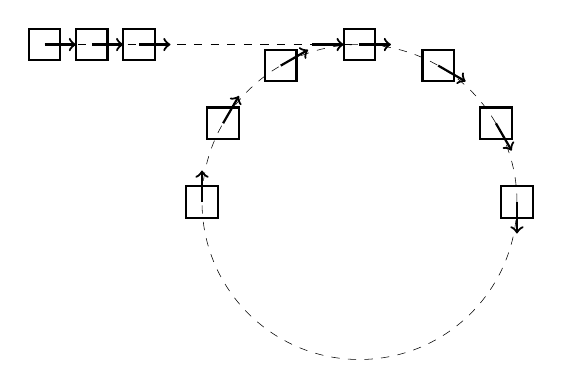
\begin{tikzpicture}[scale=2]
  % trace
  \draw[dashed, very thin] (-2cm, 1cm) -- (0, 1cm);
  \draw[dashed, very thin] (0,0) circle [radius=1cm];

  % leading nodes
  \foreach \x in {-2, -1.7, ..., -1.4} {
    \draw[thick] (\x cm, 1cm) +(-0.1, -0.1) rectangle ++(0.1, 0.1);
    \draw[thick, ->] (\x cm, 1cm) -- +(0.2, 0);
  }

  % cricular starting points
  \draw[thick, ->] (-0.3cm, 1cm) -- (-0.1cm, 1cm);

  % circular nodes
  \foreach \deg/\rot in {90/0, 60/-30, 30/-60, 0/-90, 180/90, 150/60, 120/30} {
    \draw[thick] (\deg : 1cm) +(-0.1, -0.1) rectangle ++(0.1, 0.1);
    \draw[thick, ->] (\deg : 1cm) -- +(\rot : 0.2);
  }
\end{tikzpicture}
\caption{带有循环的列表}
\label{fig:circular-list}
\end{figure}

\ifx\wholebook\relax \else
\begin{thebibliography}{99}

\bibitem{fp-pearls}
Richard Bird. ``Pearls of Functional Algorithm Design''. Cambridge University Press; 1 edition (November 1, 2010). ISBN: 978-0521513388

\bibitem{slpj-book-1987}
Simon L. Peyton Jones. ``The Implementation of Functional Programming Languages''. Prentice-Hall International Series in Computer Since. Prentice Hall (May 1987). ISBN: 978-0134533339

\bibitem{moderncxx}
Andrei Alexandrescu. ``Modern C++ design: Generic Programming and Design Patterns Applied''. Addison Wesley February 01, 2001, ISBN 0-201-70431-5

\bibitem{mittype}
Benjamin C. Pierce. ``Types and Programming Languages''. The MIT Press, 2002. ISBN:0262162091

\bibitem{unplugged}
刘新宇. ``同构——编程中的数学''. 2020. \url{https://github.com/liuxinyu95/unplugged}

\bibitem{SICP}
Harold Abelson, Gerald Jay Sussman, Julie Sussman. ``Structure and Interpretation of Computer Programs, 2nd Edition''. MIT Press, 1996, ISBN 0-262-51087-1

\bibitem{okasaki-book}
Chris Okasaki. ``Purely Functional Data Structures''. Cambridge university press, (July 1, 1999), ISBN-13: 978-0521663502

\bibitem{algo-fp}
Fethi Rabhi, Guy Lapalme. ``Algorithms: a functional programming approach''. Second edition. Addison-Wesley, 1999. ISBN: 0201-59604-0

\bibitem{learn-haskell}
Miran Lipovaca. ``Learn You a Haskell for Great Good! A Beginner's Guide''. No Starch Press; 1 edition April 2011, 400 pp. ISBN: 978-1-59327-283-8

\bibitem{erlang}
Joe Armstrong. ``Programming Erlang: Software for a Concurrent World''. Pragmatic Bookshelf; 1 edition (July 18, 2007). ISBN-13: 978-1934356005

\bibitem{wiki-tail-call}
Wikipedia. ``Tail call''. \url{https://en.wikipedia.org/wiki/Tail_call}

\bibitem{sgi-stl-transform}
SGI. ``transform''. \url{http://www.sgi.com/tech/stl/transform.html}

\bibitem{poj-drunk-jailer}
ACM/ICPC. ``The drunk jailer.'' Peking University judge online for ACM/ICPC. \url{http://poj.org/problem?id=1218}.

\bibitem{Haskell-wiki}
Haskell wiki. ``Haskell programming tips''. 4.4 Choose the appropriate fold. \url{http://www.haskell.org/haskellwiki/Haskell_programming_tips}

\bibitem{wiki-dot-product}
Wikipedia. ``Dot product''. \url{https://en.wikipedia.org/wiki/Dot_product}

\end{thebibliography}

\expandafter\enddocument
\fi
